\section{Weitere Ergebnisse und Plots für \dimcomplus{3}{1} }

\begin{frame}{Unitäre Transformationen für die CDW}
\label{cdwU}
\textbf{Unitäre transformationen zur Diagonalisierung von $\FSvertexArg{\FSeaaEoMI}{\MFpsib, \MFpsi}$ und $\FSvertexArg{\FSeaaEoMI}{\MFphi_i, \MFphi_j}$:}

\begin{align*}
U_\psi(\vec{x}\vts)= \exp(- \iu \gammach t_3 \vec{q}\cdot\vec{x}\vts)
\end{align*}

\begin{align*}
U_\varphi(\vec{x}\vts)_{ij}=\frac{1}{2}\left(
\begin{array}{cccc}
	1 - \exp(-2\iu \vec q \cdot \vec x)& 0& 0& 1+\exp(-2\iu \vec q \cdot \vec x)\\
	0 & 2& 0&0\\
	0 & 0& 2&0\\
	-\iu(1+\exp(-2\iu \vec q \cdot \vec x)) & 0& 0& \iu(\exp(-2\iu \vec q \cdot \vec x)-1)\\
\end{array}
\right)_{ij}
\end{align*}
\end{frame}

\begin{frame}{Flussgleichung für QM Model mit CDW Kondensat}
	\label{cdwFlow}
	\hspace*{-1.5em}
	\begin{minipage}{\textwidth}
		\footnotesize\vspace{-0.15cm}
		\begin{align*}
			\partial_k U_k(\rho)&=12\int\! \frac{\dif^{\, 3}\!p}{(2\piu)^3}\sum_{\pm}\big[-1+\nf(\beta [E_{\psi;k}^\pm+\mu])+\nf(\beta [E_{\psi;k}^\pm-\mu])\big]\partial_k E_{\psi;k}^\pm+\notag\\[.1em]
			&\qquad\qquad\qquad\qquad\qquad +\int\! \frac{\dif^{\, 3}\!p}{(2\piu)^3}\sum_{i=0}^3\big(\tfrac{1}{2}+\nb(\beta E_{\phi,i;k})\big)\tilde{\partial}_k E_{\phi,i;k}
		\end{align*}\vspace{-0.4cm}

		\begin{align*}
			(E_{\psi;k}^\pm)^2&\stackrel{\phantom{q=0}}{=}M^2+\frac{(\vec{p}_k^{\mkern 2mu +q})^2}{2} +\frac{(\vec{p}_k^{\mkern 2mu -q})^2}{ 2}\pm\sqrt{M^2\del{\vec{p}_k^{\mkern 2mu +q}-\vec{p}_k^{\mkern 2mu -q}}^2+\frac{1}{4}\del{(\vec{p}_k^{\mkern 2mu +q})^2 -(\vec{p}_k^{\mkern 2mu -q})^2 }^2}\\
			&\stackrel{q=0}{=} M^2+\del{\vec{p}_k}^2
		\end{align*}\vspace{-0.4cm}
		\begin{align*}
			(E_{\phi;k}^{0,3})^2&\stackrel{\phantom{q=0}}{=}\frac{1}{2 }(\vec{p}_k)^2 +\frac{1}{2 }(\vec{p}_k^{\mkern 2mu+4q})^2+2U_k'(\rho) +2\rho U_k''(\rho)\,
			\pm \sqrt{4\rho^2 U_k''(\rho)^2+\frac{1}{4}\del{(\vec{p}_k^{\mkern 2mu+4q})^2-(\vec{p}_k)^2 }^2}\\
			&\stackrel{q=0}{=}\del{\vec{p}_k}^2+2U_k'(\rho)+2\rho (U_k''(\rho)\pm|U_k''(\rho)|)\\
			(E_{\phi;k}^{1})^2&=(E_{\phi;k}^{2})^2\stackrel{\phantom{q=0}}{=}(\vec{p}_k)^2+2U_k'(\rho)\stackrel{q=0}{=}\del{\vec{p}_k}^2+2U_k'(\rho)
		\end{align*}\vspace{-0.4cm}
		\begin{align*}
			\vec{p}_k^{\mkern 2mu q}&\equiv\del{\vec p + {\vec q/ 2}}\lambda_k\del{|\vec p + {\vec q/ 2}|}\qquad\text{und}\qquad
			M^2\equiv \frac{1}{4} h^2 \Delta^2=\frac{h^2}{2}\rho
		\end{align*}
	\end{minipage}
	
\end{frame}


\begin{frame}{Das Problem mit naiver Parameter-Fixierung}
	\begin{center}
		\begin{overlayarea}{\framewidth}{6.2cm}
				\only<1|handout:1>{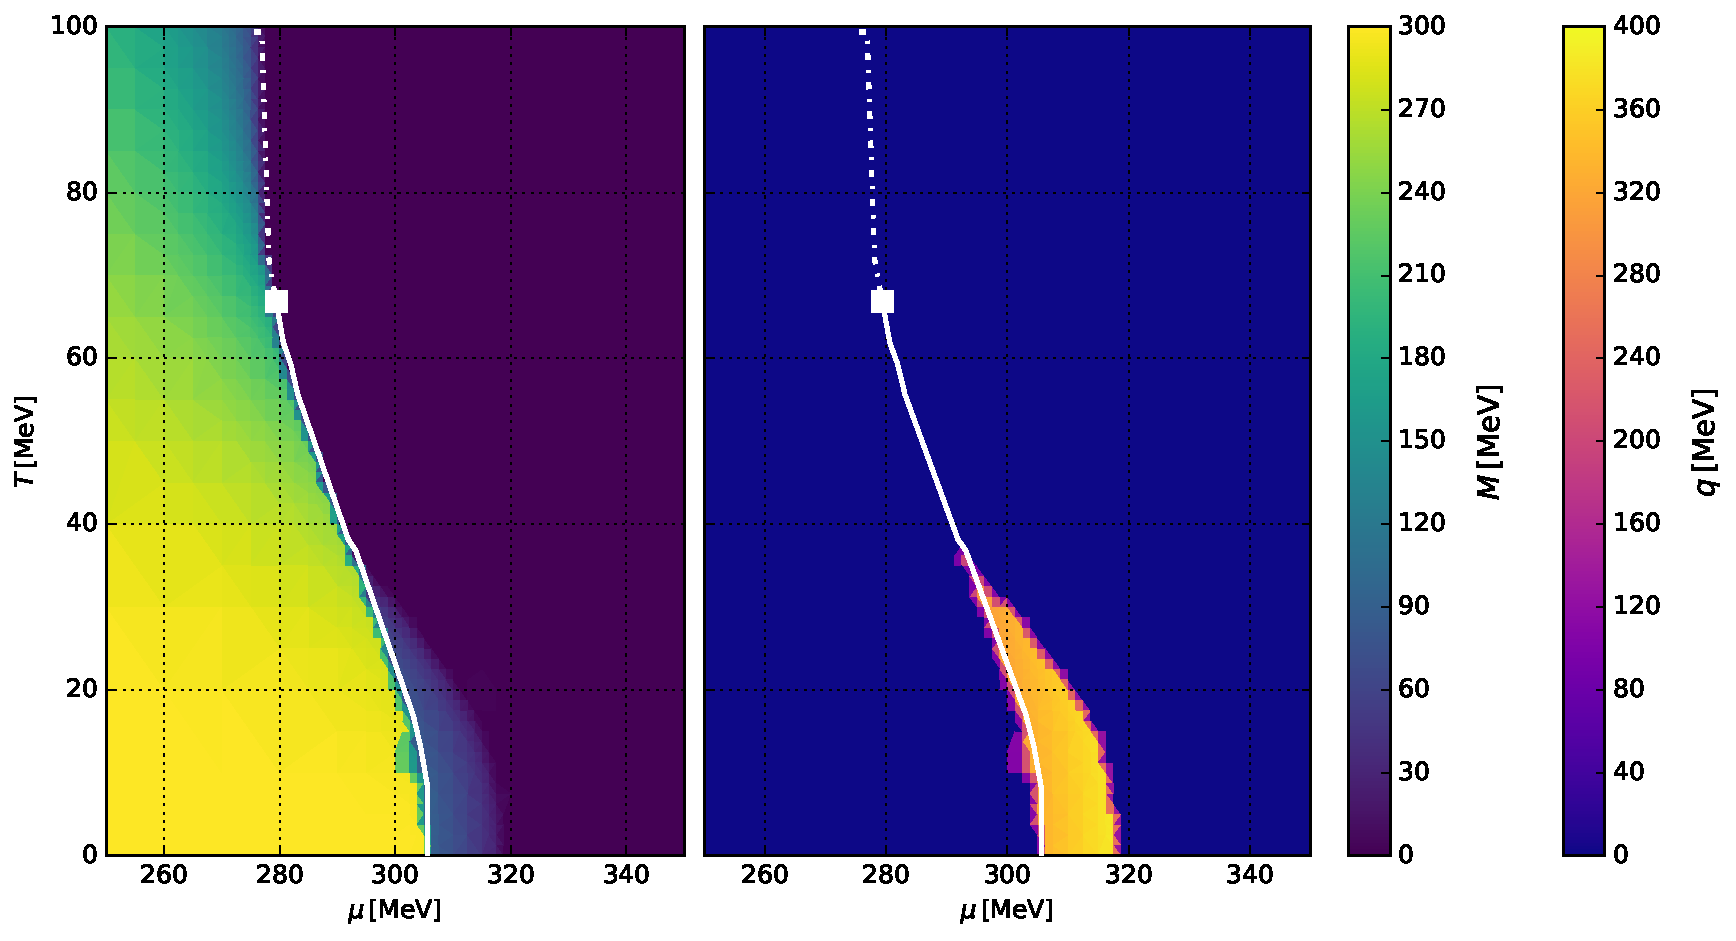
\includegraphics[width=\framewidth]{figures/eMFAinhomo400.pdf}}
				\only<2|handout:2>{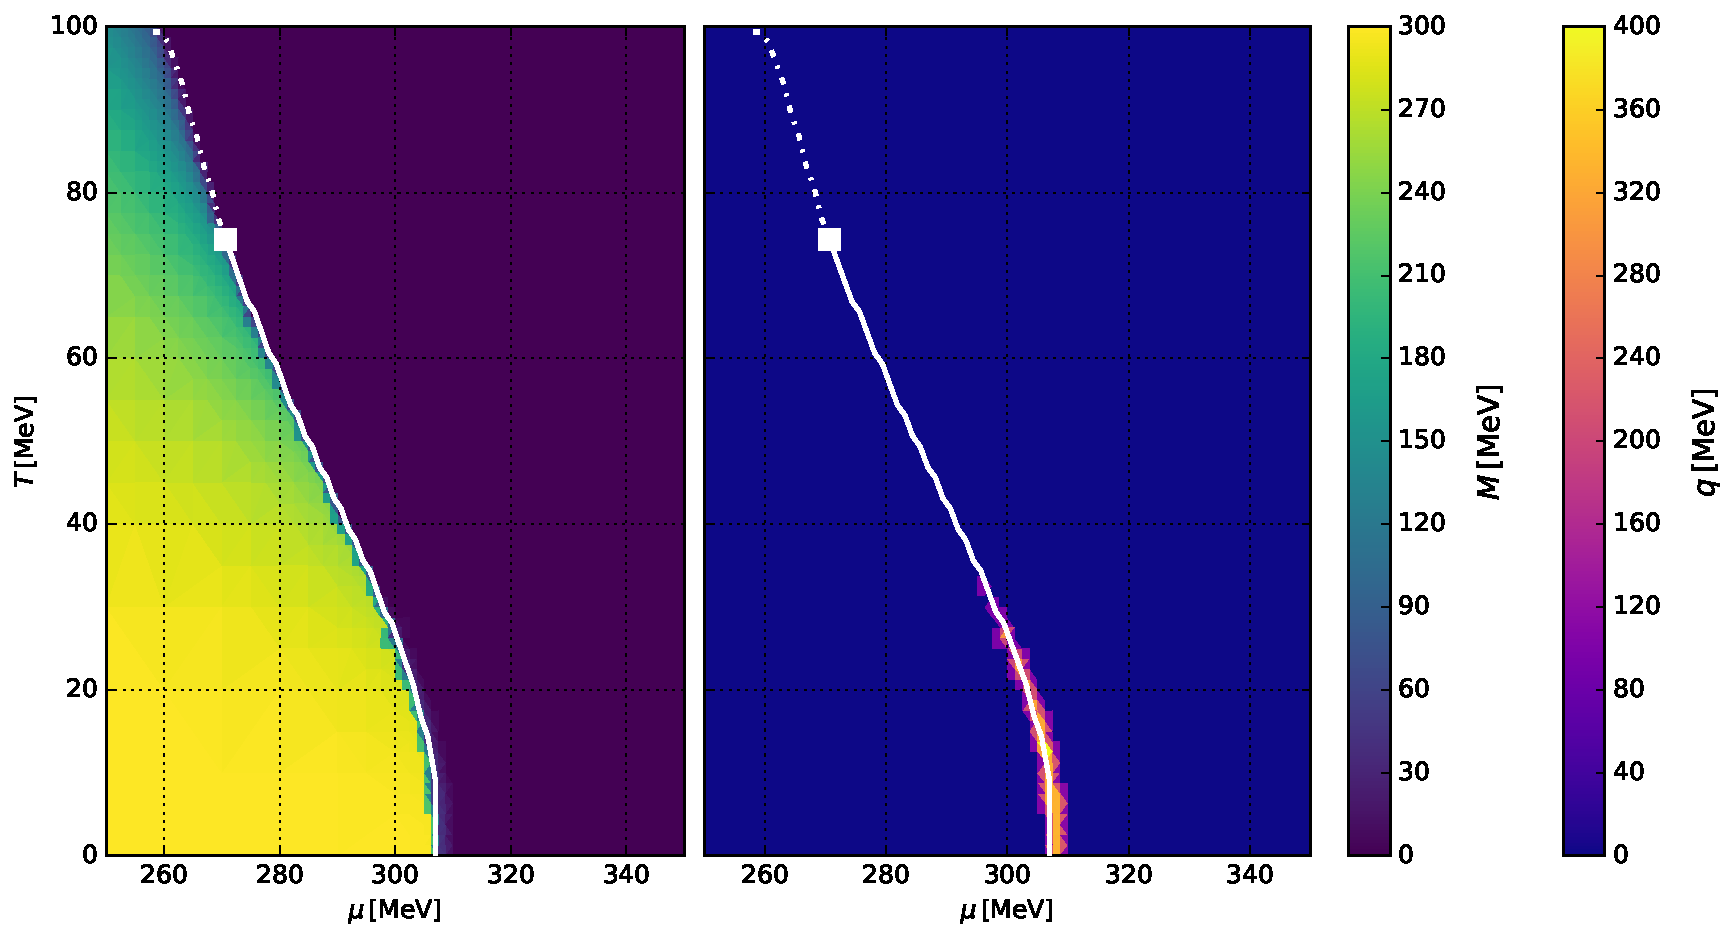
\includegraphics[width=\framewidth]{figures/eMFAinhomo450.pdf}}
				\only<3|handout:3>{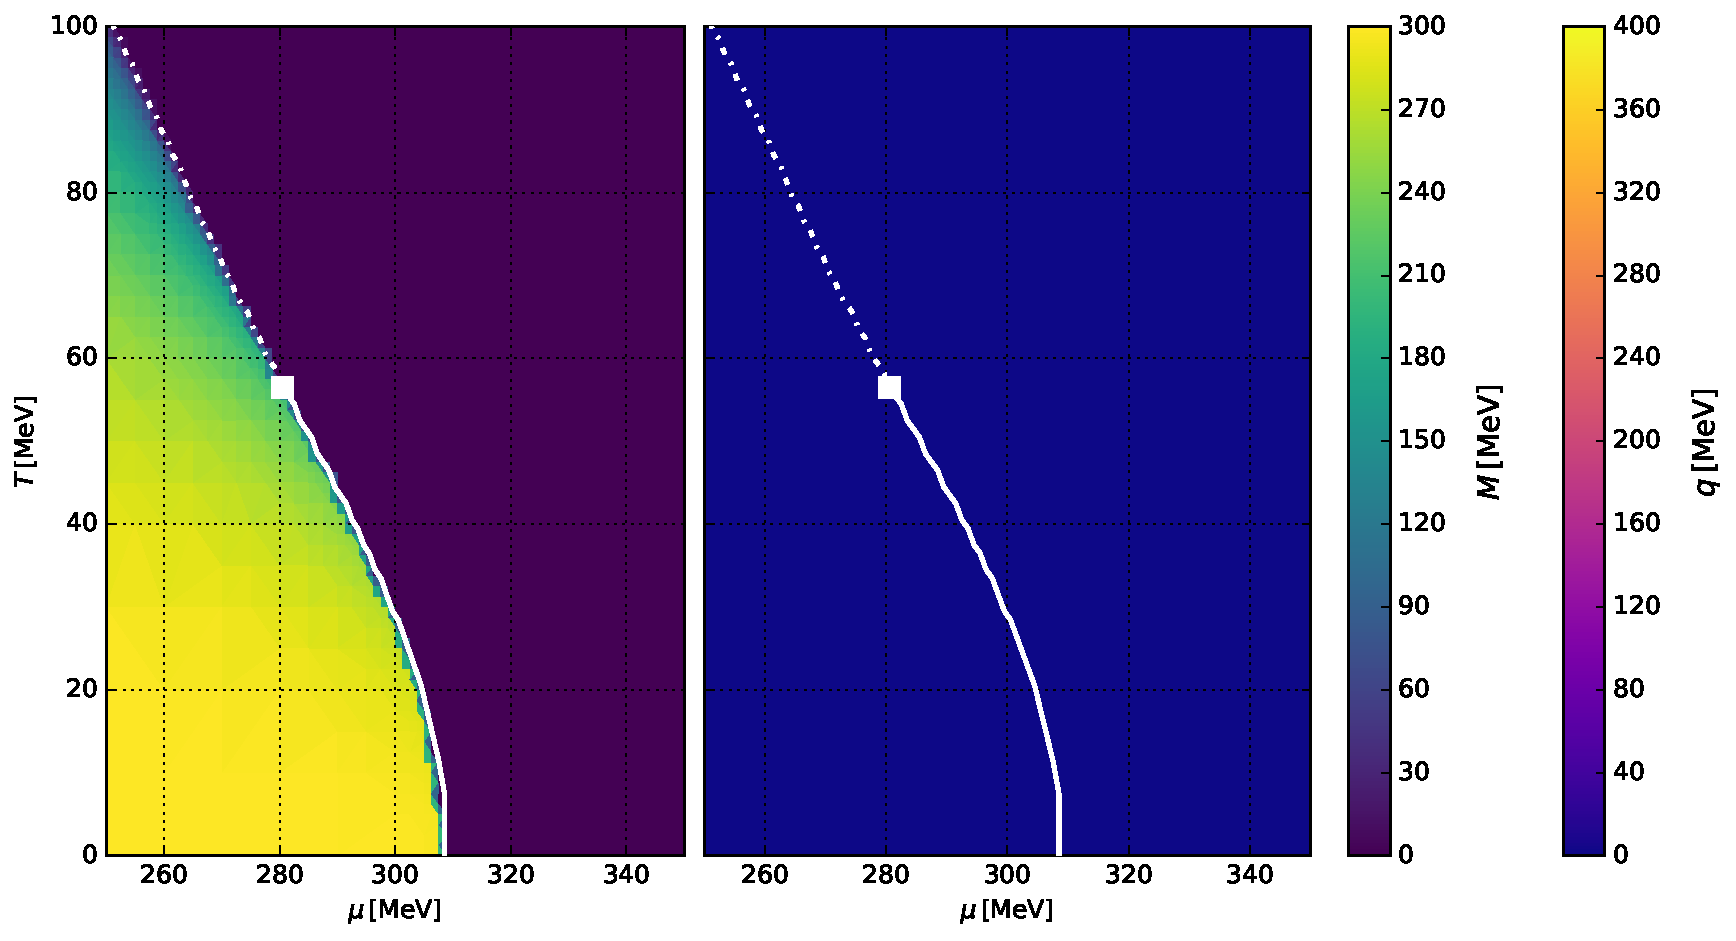
\includegraphics[width=\framewidth]{figures/eMFAinhomo500.pdf}}
		\end{overlayarea}
	\end{center}
\end{frame}
